\documentclass[11pt]{article}
\usepackage[letterpaper,margin=2cm]{geometry}
\usepackage[utf8]{inputenc}
\usepackage[spanish , english]{babel}
\usepackage{amssymb, amsmath, amsbsy, amsfonts}
\usepackage{upgreek}
\usepackage{graphicx}
\usepackage{multicol}
\usepackage{color}
\usepackage{caption}
\usepackage{hyperref}
\renewcommand{\figurename}{Fig.}
\renewcommand{\tablename}{Tab.}
\setlength{\columnsep}{5mm}
\title{\textbf{Medicion Directa: Resistencia Electrica}\\{\textcolor{black}{Murillo Bernal Miguel\\Mamani Calle Alex}}}
\author{LAB123A-06-01, Laboratorio de Física II, INF-FCPN-UMSA}
\date{15/09/2023}
\begin{document}
    \maketitle
    \selectlanguage{spanish}
    \begin{abstract}
        \noindent Se aplico la teoría de grandes muestras sobre 40 mediciones realizadas a 2 resistencias con valor nominal
        de $2.2[M\Omega]$ para obtener su valor real: $R = 2.23\pm0.02\left[ M\Omega \right]; N.C. = 95\% $
        y verificar mediante una prueba de hipótesis nula que su valor nominal es correcto. \\
        Palabras clave: Resistencia, Hipótesis nula, Teoría de Grandes muestras, Medición Directa.
    \end{abstract}
    \selectlanguage{english}
    \begin{abstract}
        \noindent The big samples theory was applied over 40 samples taken from 2 different resistors
        with a nominal value of $2.2[M\Omega]$ to get his real value, which ended being:
        $2.23\pm0.02\left[ M\Omega \right]; N.C. = 95\% $.And verify by a null hypothesis
        test that the nominal value written was correct. \\

        Keywords: Resistor, Null Hypothesis, Big Sample Theory, Direct Measure
    \end{abstract}
%%%%%%
    \begin{multicols}{2}
        \section{\textbf{\textcolor{black}{Introdución}}}
        \noindent El valor de una resistencia esta determinada por un codigo de colores impreso
        sobre su superficie, sin embargo dicho valor puede no siempre puede ser correcto, en el
        presente informe se utiliza la teoria de grandes muestras asi como la prueba de hipotesis
        nula sobre las mediciones obtenidas de 2 Resistencias distintas pero del mismo valor
        nominal de 2.2[$M\Omega$] bajo la hipotesis de que este valor es correcto

        \section{\textbf{\textcolor{black}{Objetivos}}}

        \subsection{\textcolor{black}{Objetivo general}}
        \noindent Evaluar y comprender la resistencia eléctrica de un material o componente
        específico mediante mediciones directas

        \subsection{\textbf{\textcolor{black}{Objetivo específico}}}
        \noindent
        \begin{itemize}
            \item Expresar correctamente el resultado para la resistencia eléctrica e incertidumbre
            al nivel de confianza del 95\%
            \item Realizar una prueba de hipótesis nula para la resistencia eléctrica experimental frente al nominal
            por código de colores al nivel de confianza dado
            tanto para los grupos pares como impares.
        \end{itemize}


        \section{\textbf{\textcolor{black}{Marco Metodológico}}}
        Se pretende medir el valor real de una resistencia frente a su valor nominal dado por el código de colores impreso en esta
        mediante una prueba de hipótesis nula frente al valor obtenido de las mediciones.


        \section{\textbf{\textcolor{black}{Marco Experimental}}}

        \subsection{\textbf{\textcolor{black}{Introducción}}}
        \noindent Se utilizó 2 Resistencias con un valor nominal de: $2.2 [M\Omega]$
        \begin{center}
            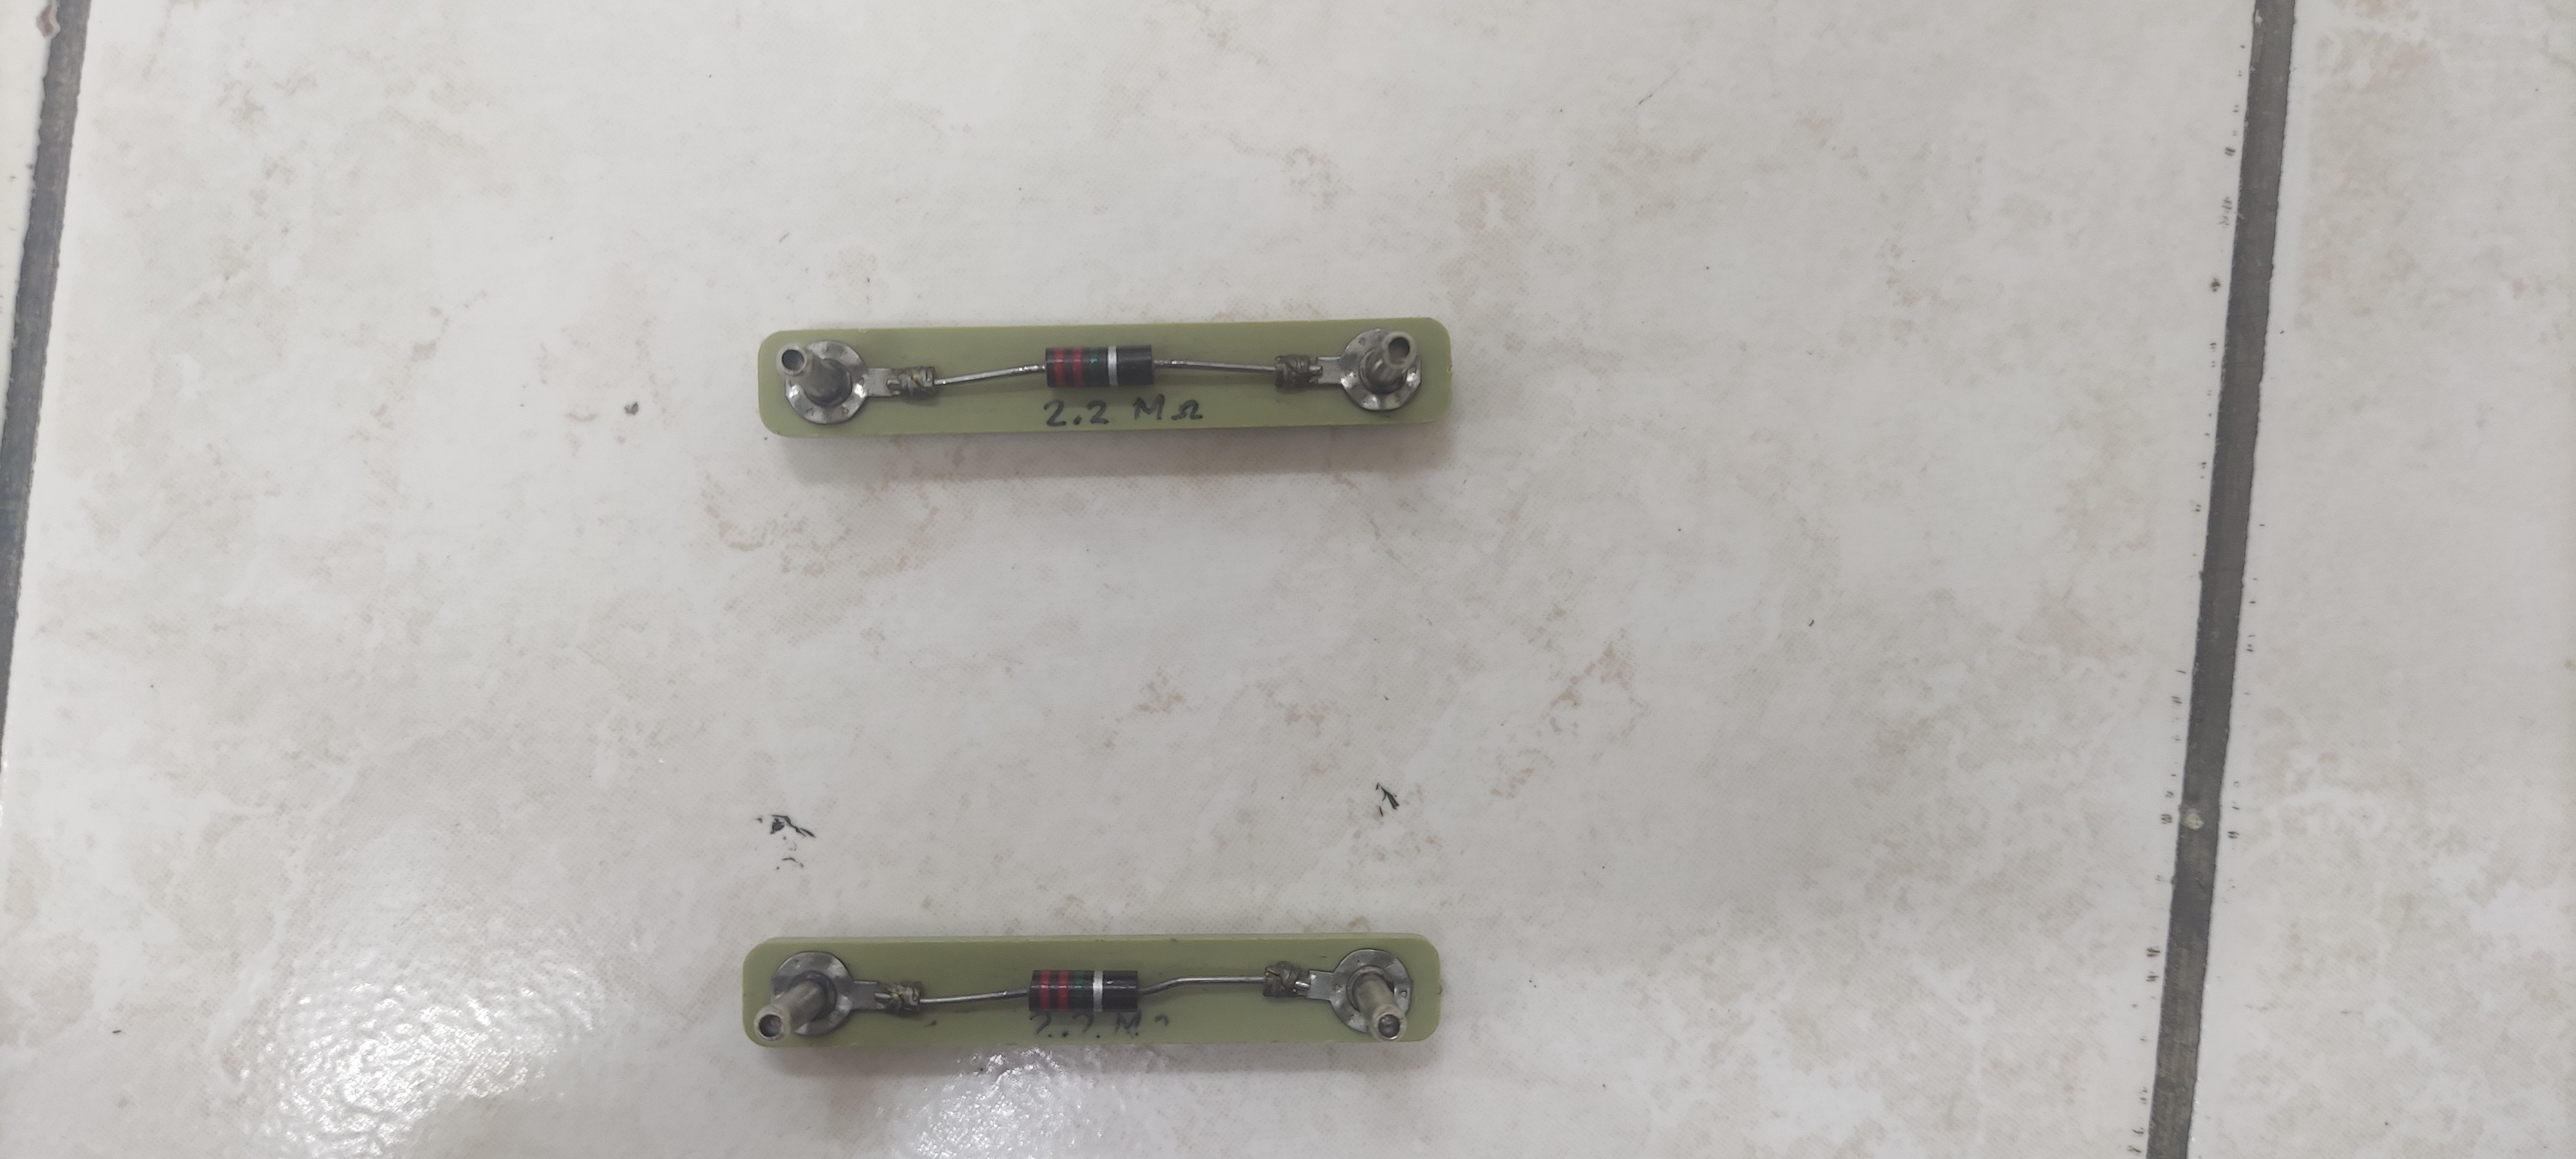
\includegraphics[width=0.4\textwidth]{img-1/res}
            \captionof{figure}{Se observa las 2 resisitencias utilizadas durante la realizacion del experimento.\label{fig01}}
        \end{center}
        \noindent  Ambas Resistencias se posicionaron de manera paralela en un punto arbitrario
        sobre una placa perforada.
        \begin{center}
            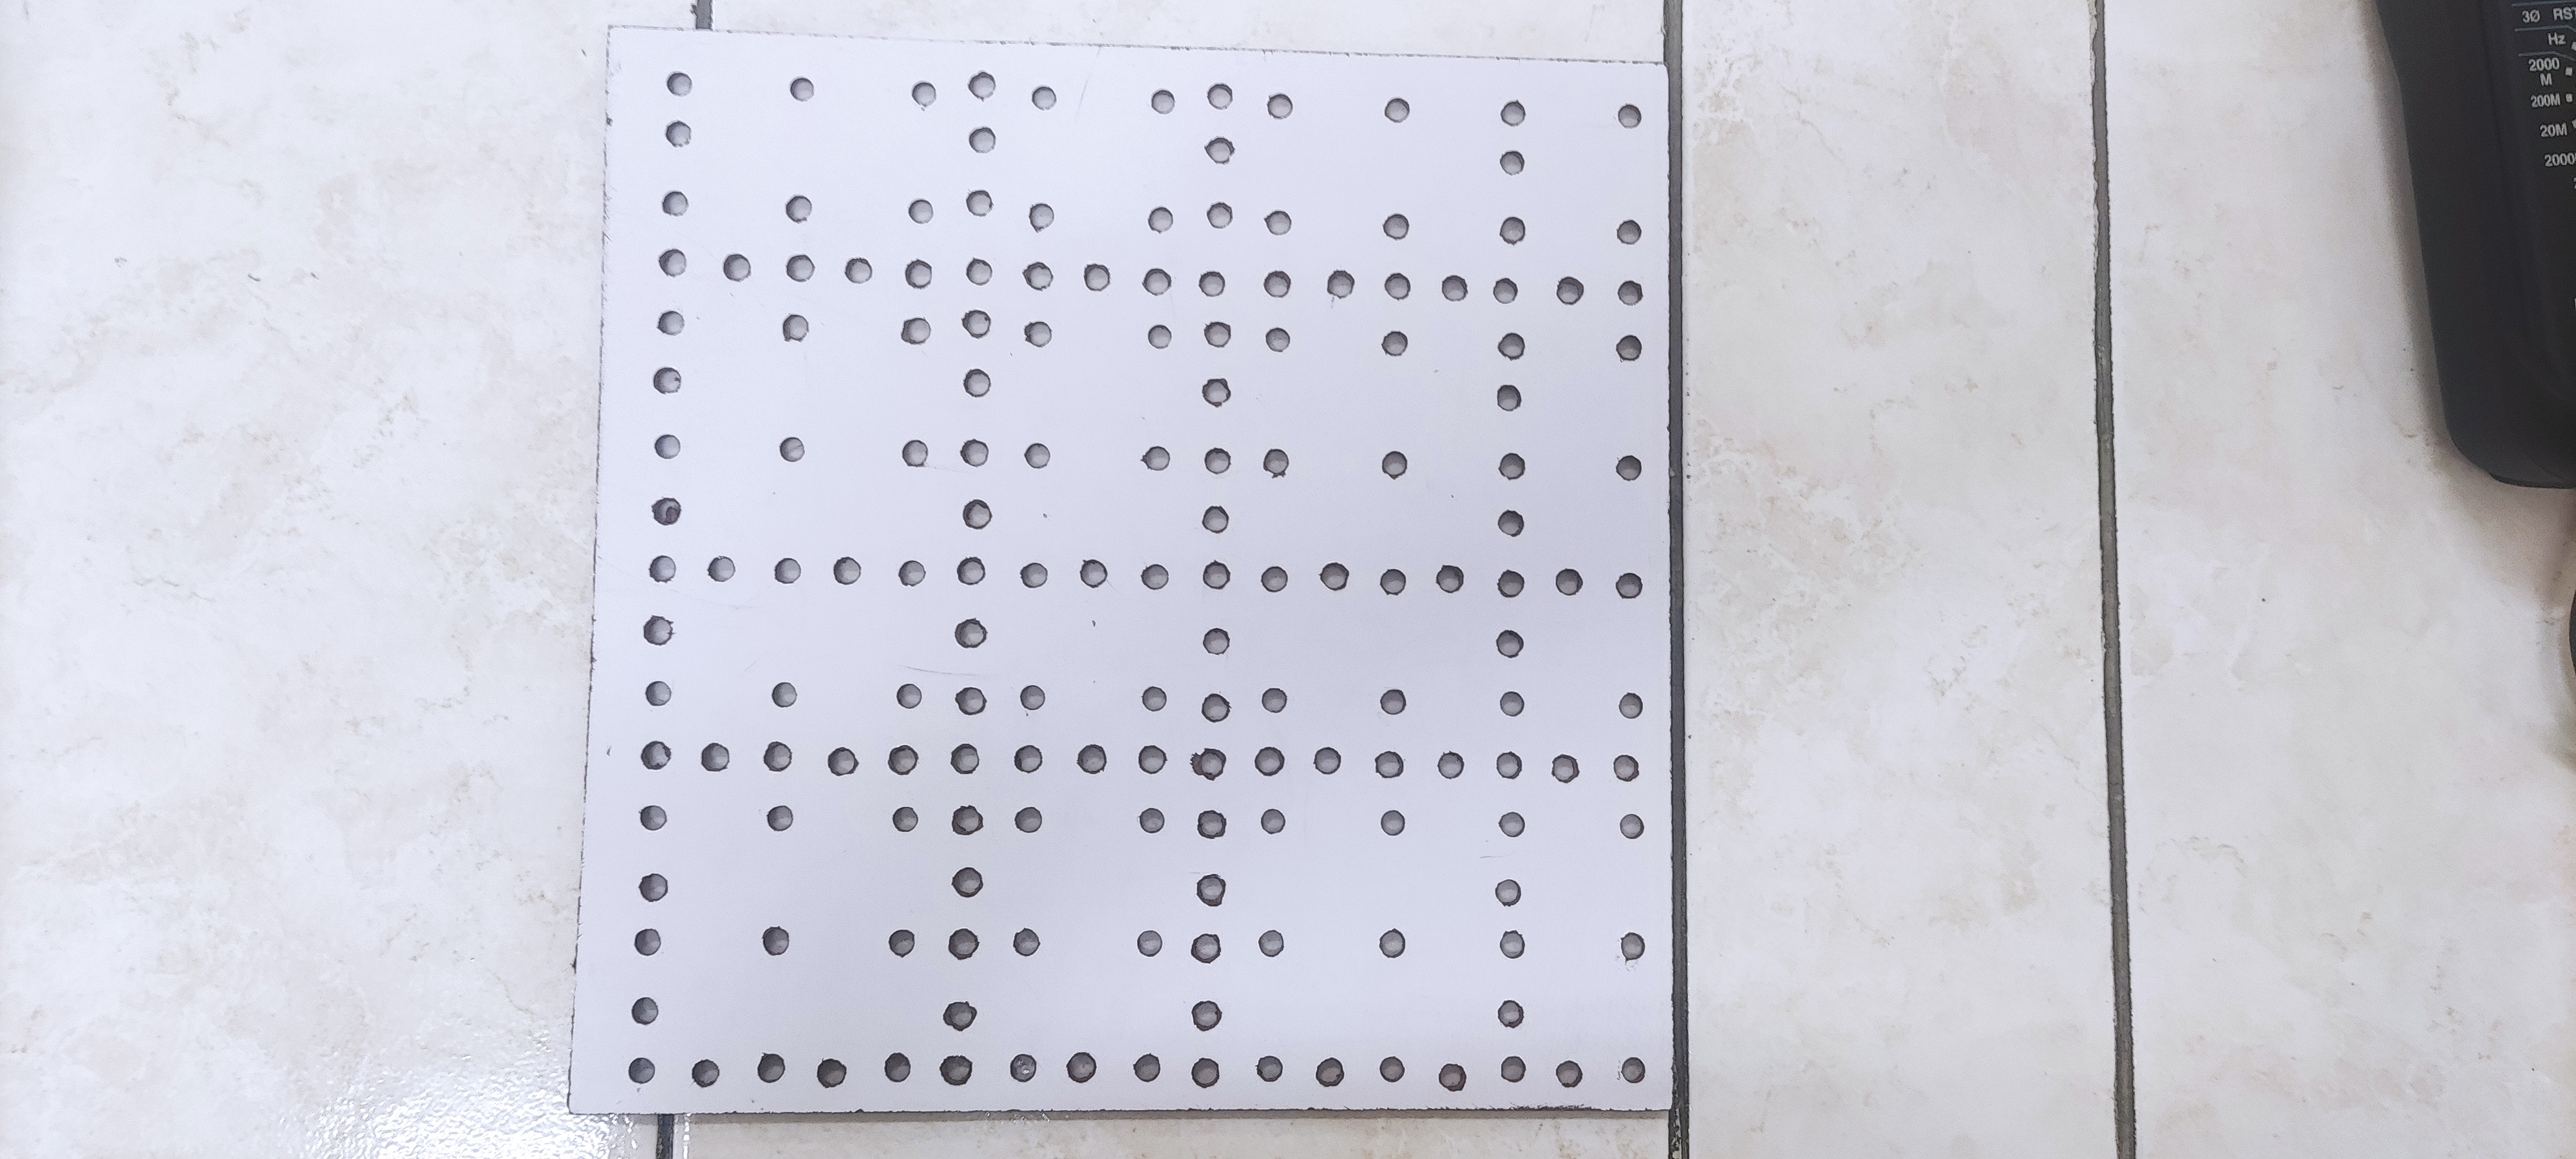
\includegraphics[width=0.4\textwidth]{img-1/board}
            \captionof{figure}{Se observa la placa perforada utilizada durante la realizacion del experimento.\label{fig02}}
        \end{center}
        \noindent Posteriormente se procede a la medición de cada resistencia de manera individual mediante el uso
        de un multímetro.
        \begin{center}
            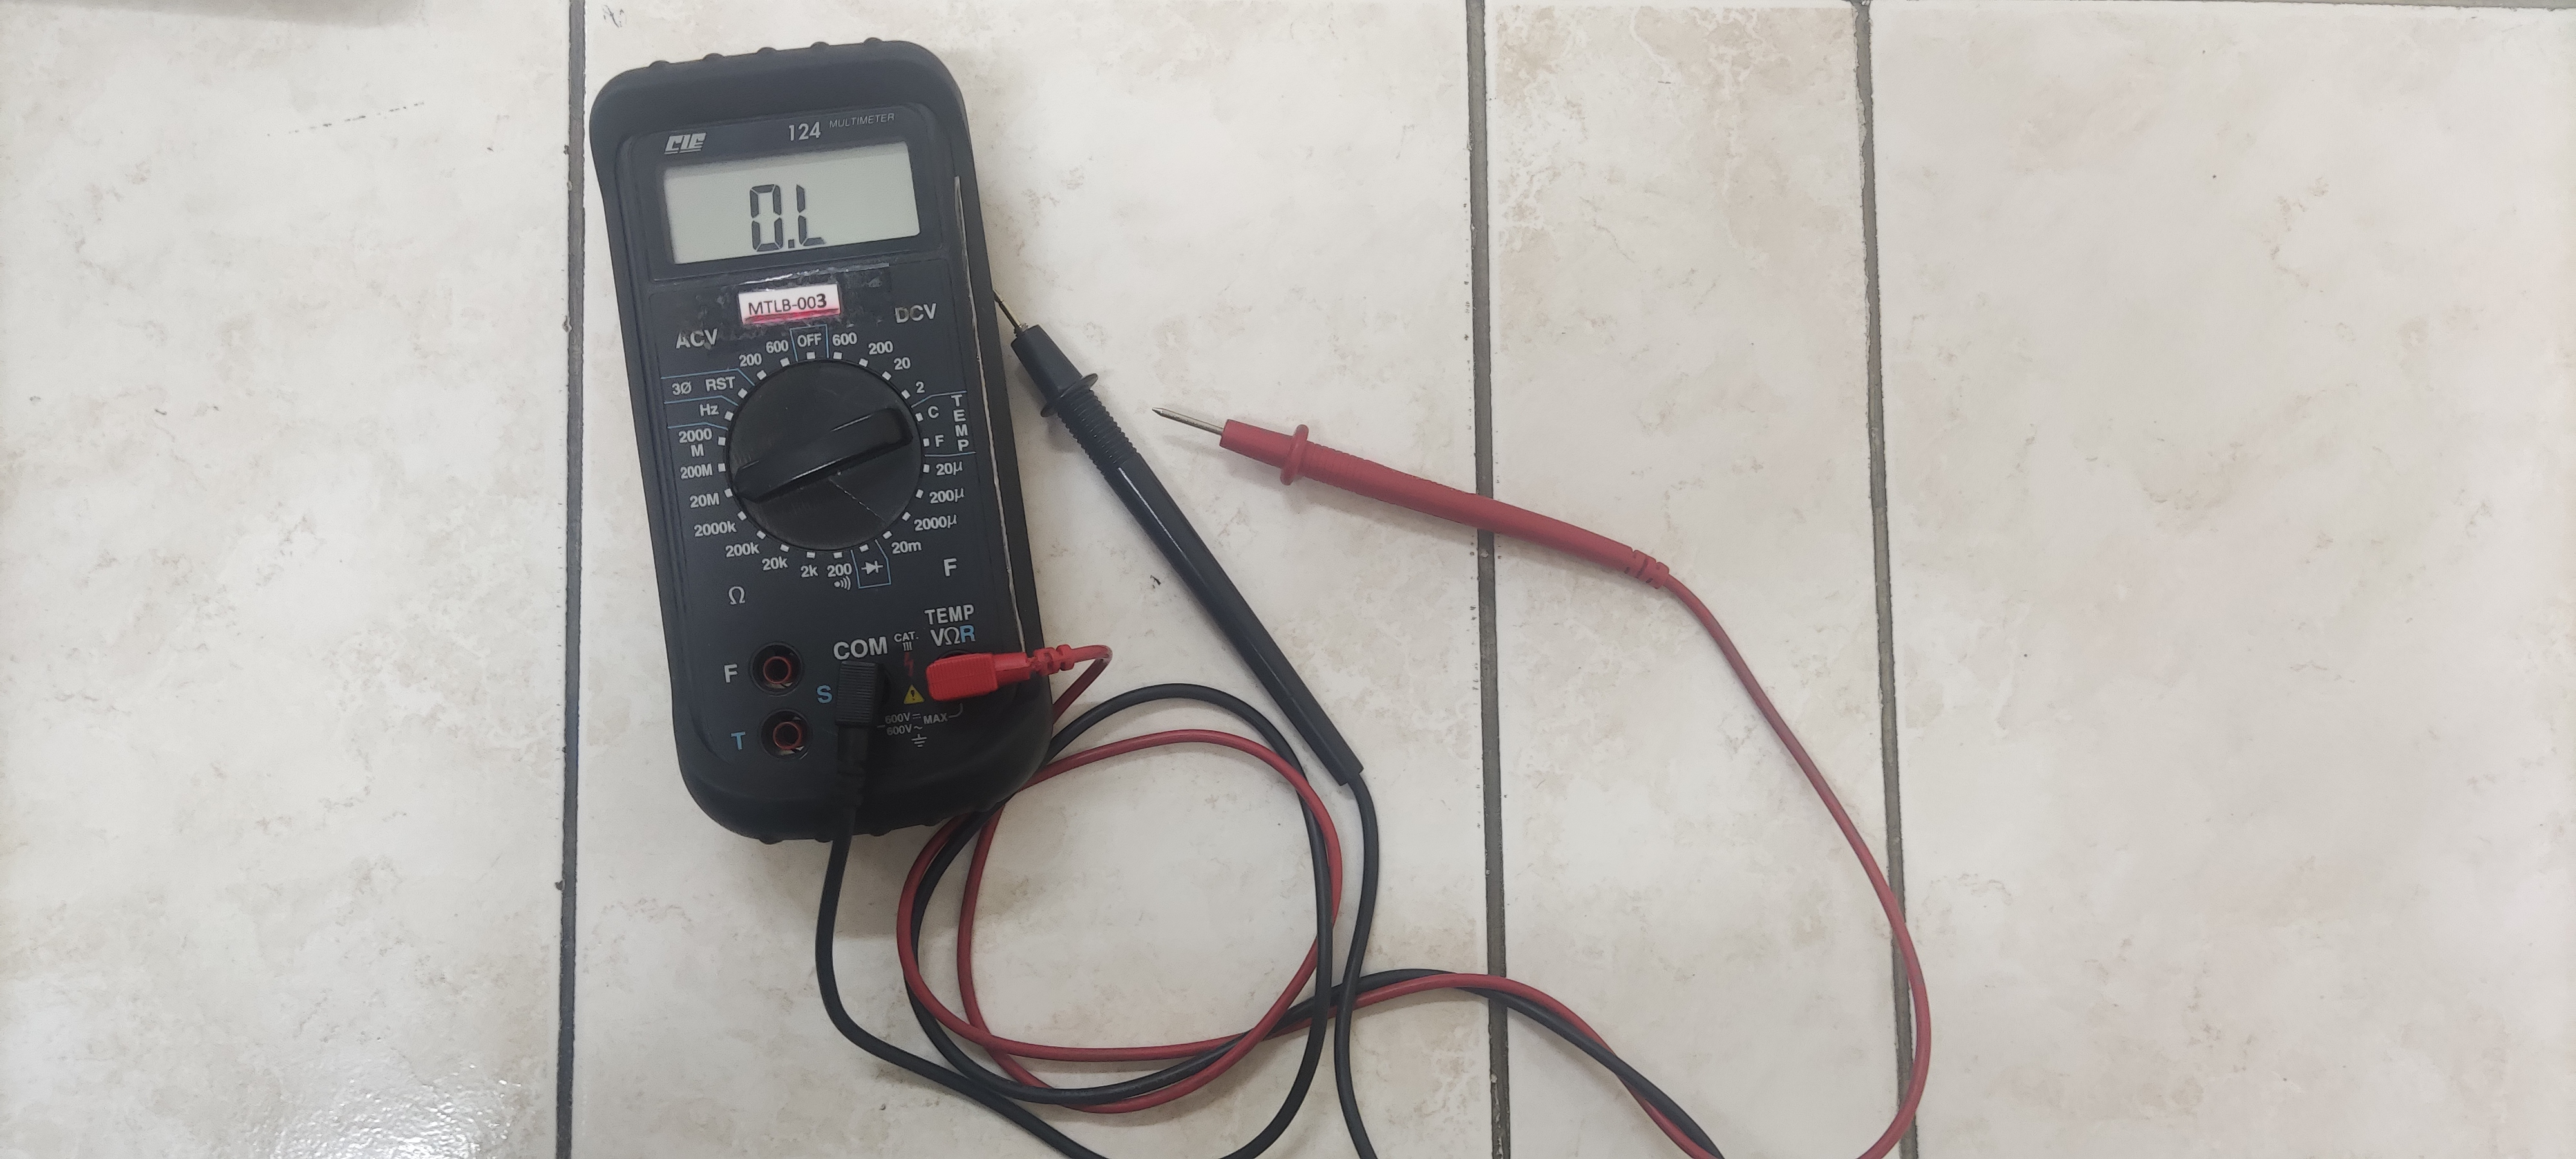
\includegraphics[width=0.4\textwidth]{img-1/multimeter}
            \captionof{figure}{Se observa el multimetro utilizado durante la realizacion del experimento.\label{fig03}}
        \end{center}
        \noindent Obteniendo asi el siguiente montaje
        \begin{center}
            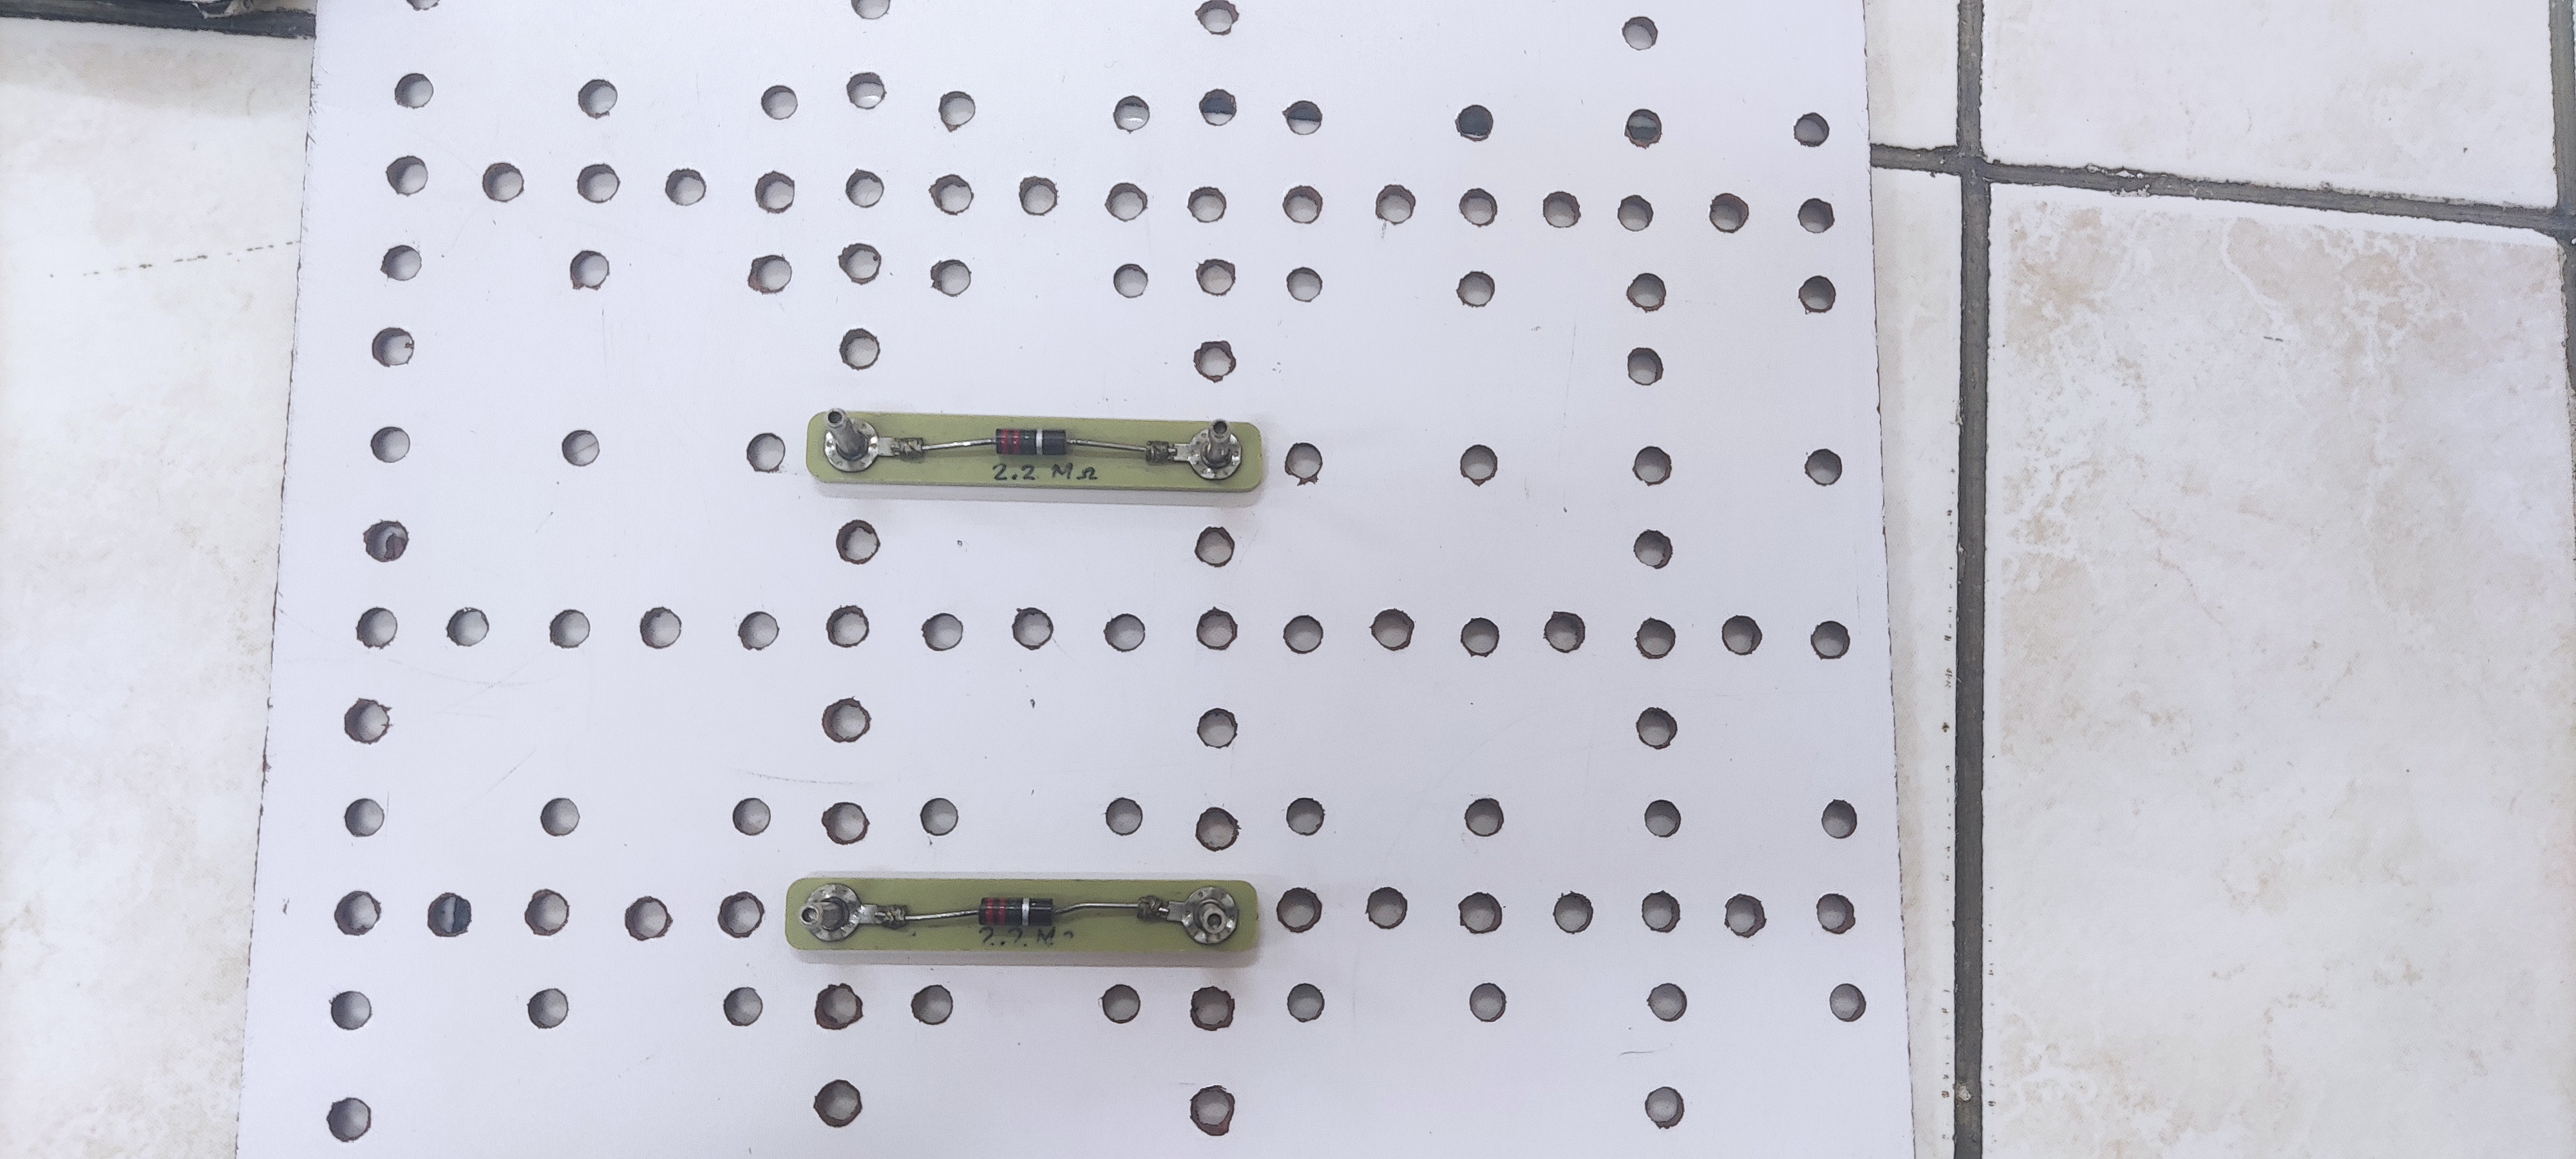
\includegraphics[width=0.4\textwidth]{img-1/setup}
            \captionof{figure}{Se observa el montaje utilizado durante la realizacion del experimento.\label{fig04}}
        \end{center}

        \subsection{\textbf{\textcolor{black}{Datos Experimentales}}}
        \noindent Para obtener las mediciones se posicionas las agujas del multímetro de manera
        que realicen contacto con los polos de la resistencia de manera individual

        \begin{center}
            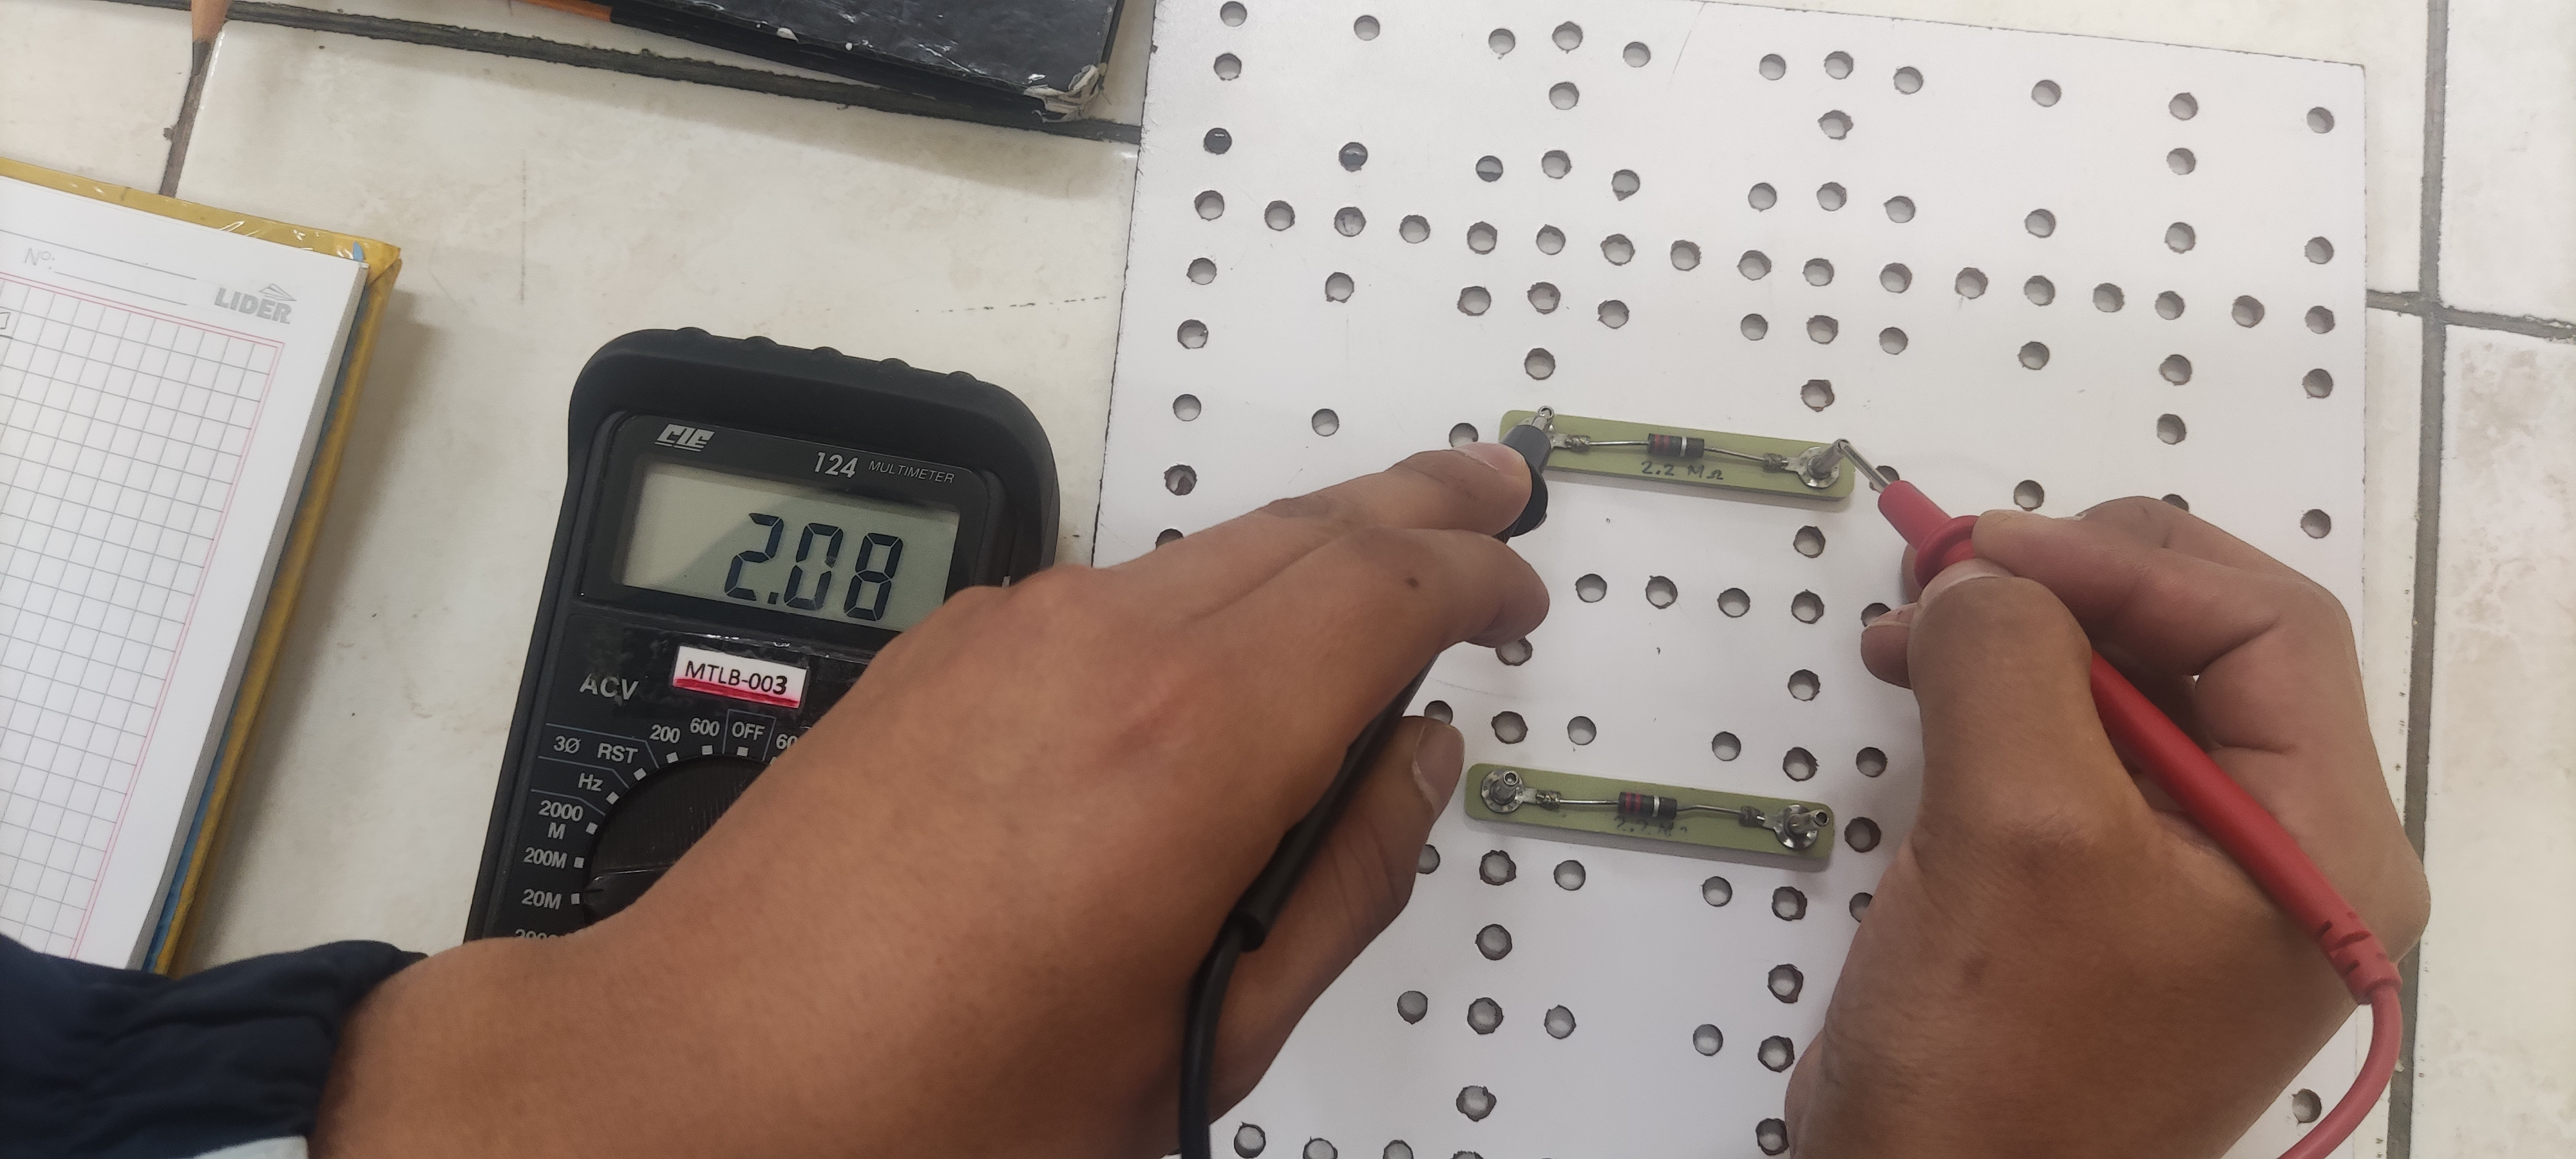
\includegraphics[width=0.4\textwidth]{img-1/med1}
            \captionof{figure}{Se observa la colocacion de los instrumentos para la medicion de la primera resistencia\label{fig05}}
        \end{center}
        \begin{center}
            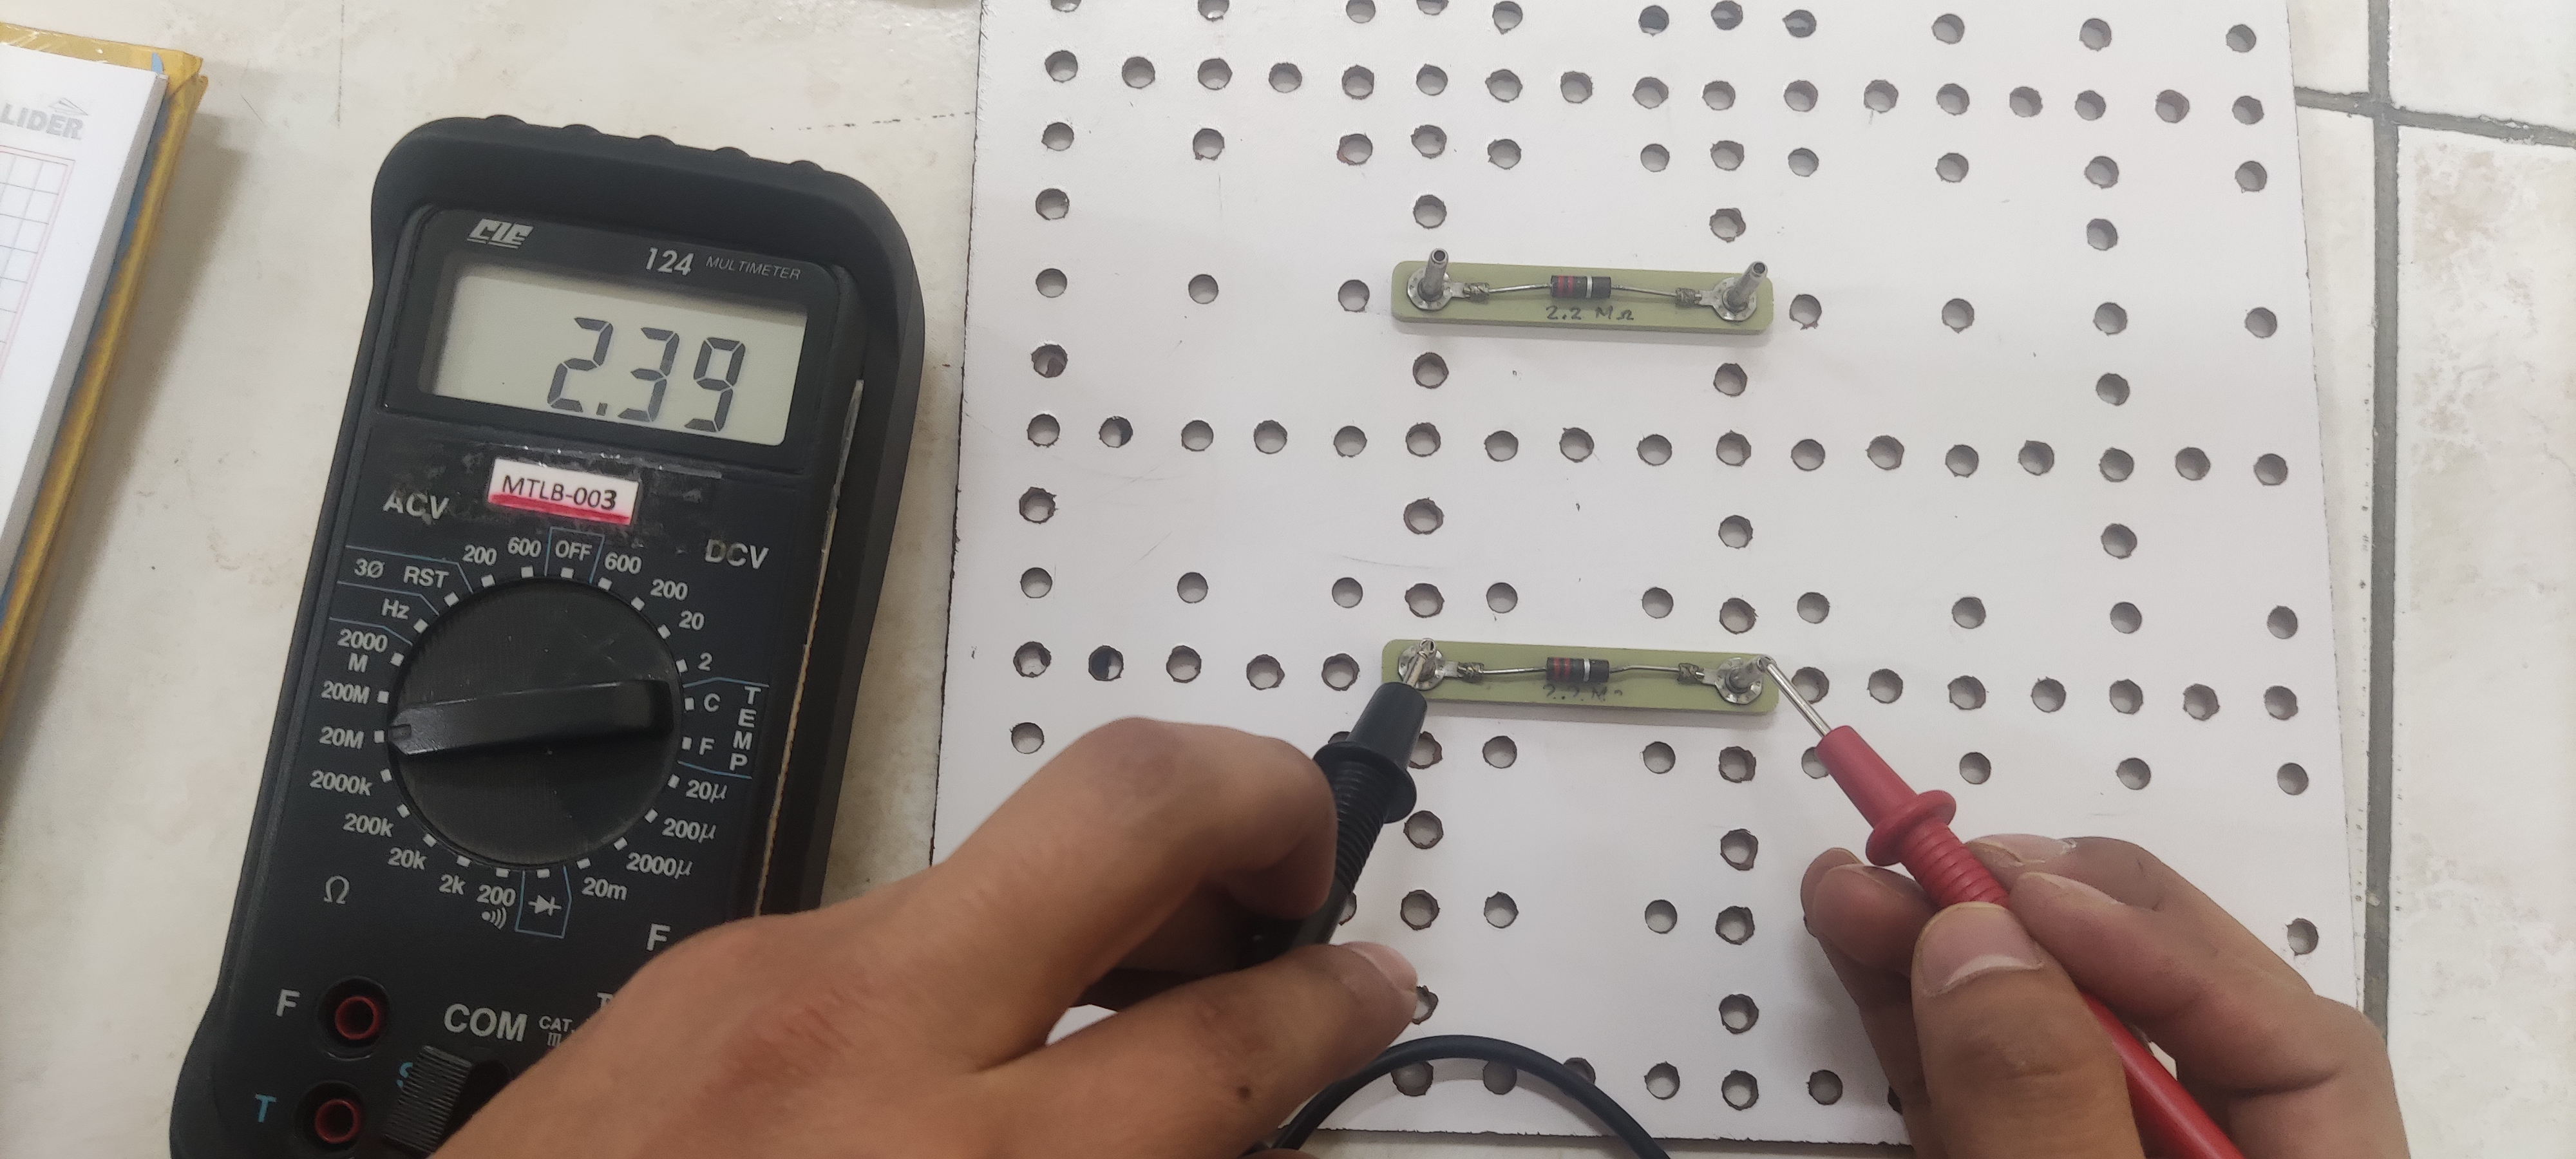
\includegraphics[width=0.4\textwidth]{img-1/med2}
            \captionof{figure}{Se observa la colocacion de los instrumentos para la medicion de la segunda resistencia\label{fig06}}
        \end{center}
        Como Resultado de las mediciones se obtuvieron los datos de la Figura\ref{fig07}:
        \begin{center}
            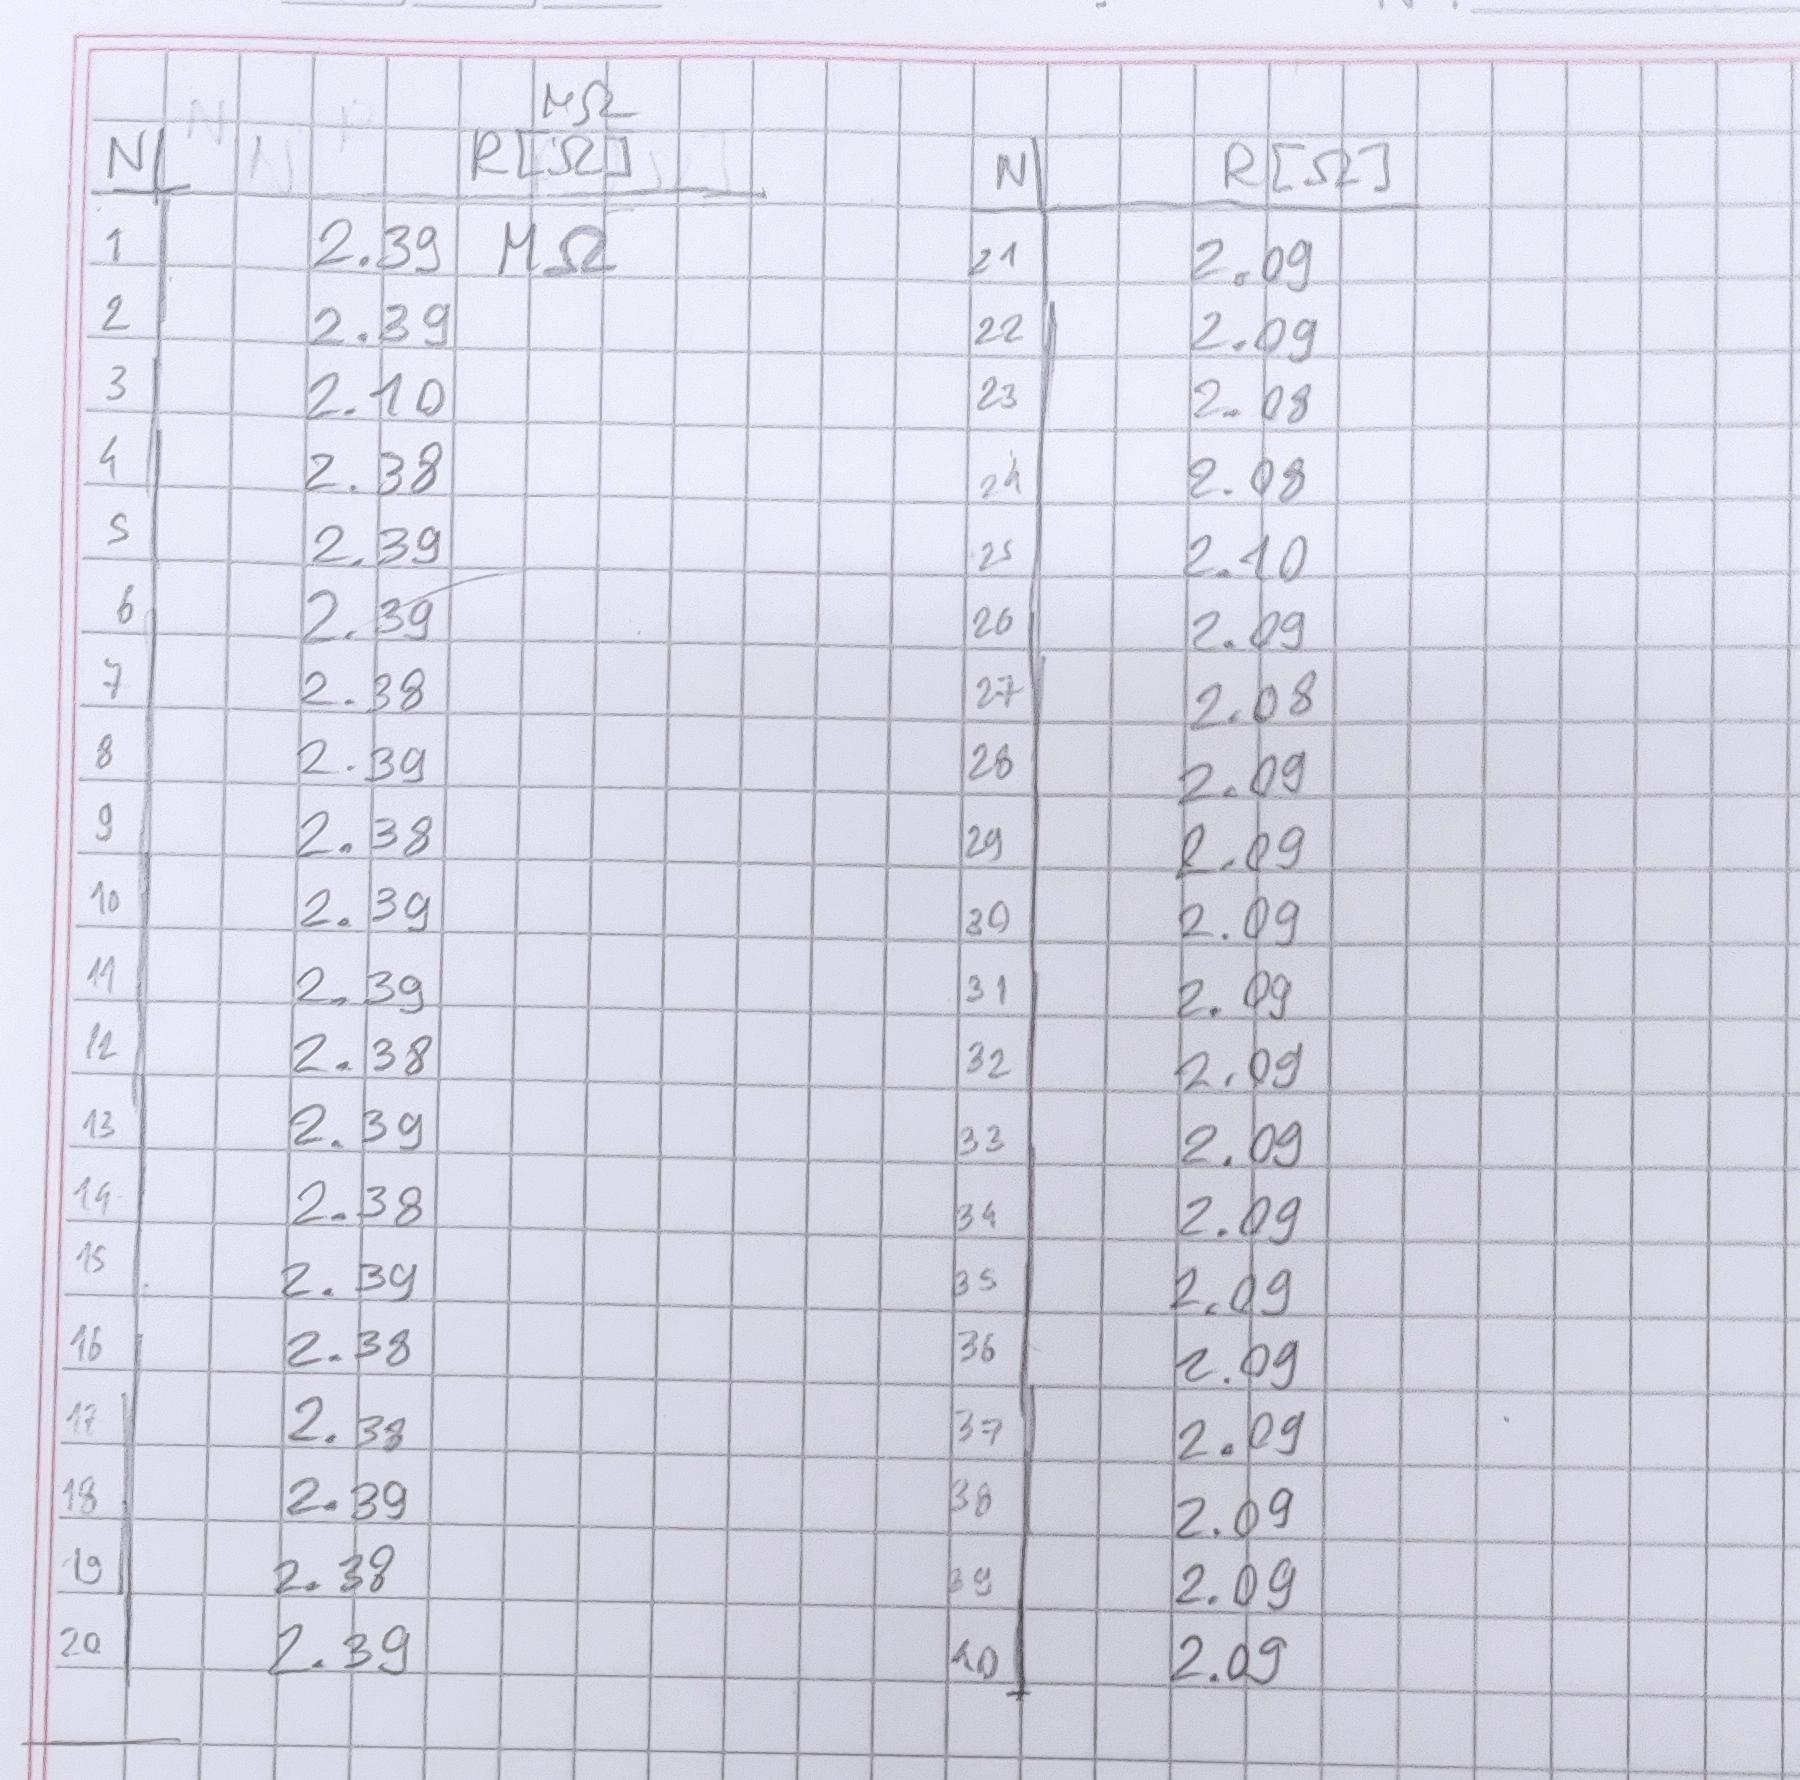
\includegraphics[width=0.4\textwidth]{img-1/mediciones}
            \captionof{figure}{Se observa el borrador de las mediciones obtenidas en el laboratorio\label{fig07}}
        \end{center}
        
        Los cuales estan transcritos en la Tabla\ref{t1}

        \begin{center}
            \begin{tabular}{|c|c||c|c|}
                \hline
                N  & R[$M\Omega$] & N  & R[$M\Omega$] \\[0,1cm]
                \hline \hline
                1  & 2.39 & 21 & 2.09         \\ \hline
                2  & 2.39 & 22 & 2.09         \\ \hline
                3  & 2.10 & 23 & 2.08         \\ \hline
                4  & 2.38 & 24 & 2.08         \\ \hline
                5  & 2.39 & 25 & 2.10         \\ \hline
                6  & 2.39 & 26 & 2.09         \\ \hline
                7  & 2.38 & 27 & 2.08         \\ \hline
                8  & 2.39 & 28 & 2.09         \\ \hline
                9  & 2.38 & 29 & 2.09         \\ \hline
                10 & 2.39 & 30 & 2.09         \\ \hline
                11 & 2.39 & 31 & 2.09         \\ \hline
                12 & 2.38 & 32 & 2.09         \\ \hline
                13 & 2.39 & 33 & 2.09         \\ \hline
                14 & 2.38 & 34 & 2.09         \\ \hline
                15 & 2.39 & 35 & 2.09         \\ \hline
                16 & 2.38 & 36 & 2.09         \\ \hline
                17 & 2.38 & 37 & 2.09         \\ \hline
                18 & 2.39 & 38 & 2.09         \\ \hline
                19 & 2.38 & 39 & 2.09         \\ \hline
                20 & 2.39 & 40 & 2.09         \\ \hline
            \end{tabular}
            \captionof{table}{Se muestra en la tabla los valores experimentales medidos a partir de un multímetro digital.}
            \label{t1}
        \end{center}
        \section{\textbf{\textcolor{black}{Resultados y análisis}}}
        \noindent Se utiliza el lenguaje de programación R para el análisis de los datos.
        Para ello primero cargamos los datos en el Lenguaje, y obtenemos la media, desviación
        estándar, y el histograma como producto de la ejecucion del codigo en la Figure\ref{fig8}.
        \begin{center}
            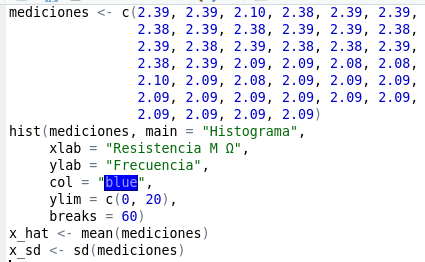
\includegraphics[width=0.4\textwidth]{img-1/code1}
            \captionof{figure}{Codigo en R para analizar los datos\label{fig8}}
        \end{center}

        \begin{center}
            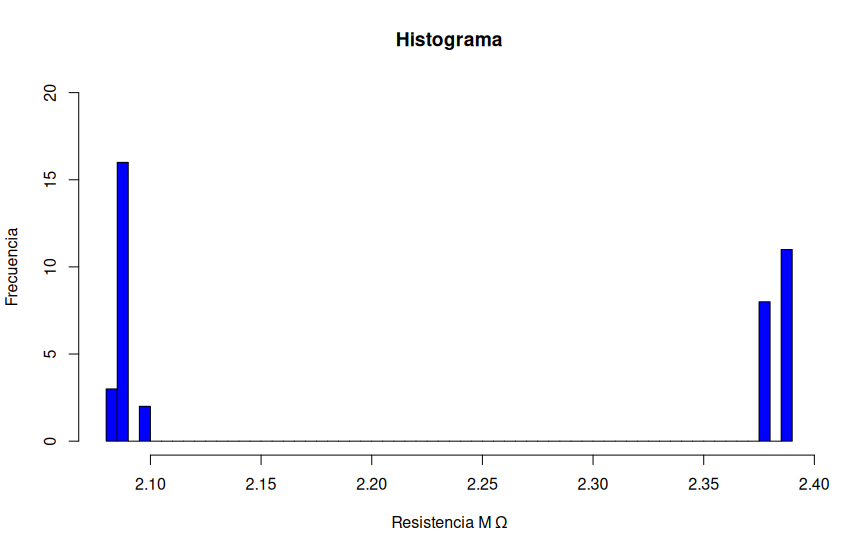
\includegraphics[width=0.4\textwidth]{img-1/hist}
            \captionof{figure}{Histograma de los datos\label{fig9}}
        \end{center}

        \begin{center}
            \begin{tabular}{||c|c|c||}
                \hline
                n  & $\bar{x}$ & $\sigma_x$  \\[0,1cm]
                \hline \hline
                40  & 2.23 & 0.1499143       \\ \hline
            \end{tabular}
            \captionof{table}{Valores obtenidos del analisis con R}
            \label{t2}
        \end{center}

        Suponemos una hipótesis $H_0$ que el valor de las resistencias es de 2.2[$M\Omega$]
        y Una Hipotesis Alternativa $H_1$ que el valor de la Resistencia es distinto, es decir:

        \begin{equation}
            H_0: \mu = \mu_0 \\
            H_1: \mu \neq \mu_0
        \end{equation}

        Donde $\mu_0$ es el valor esperado 2.2[$M\Omega$] y $\mu$ es el valor de las resistencias.

        De ahí se sigue que con un nivel de confianza del $\alpha = 95\%$ tenemos que:
        \begin{equation}
            P[-z_{1- \frac{\alpha}{2}} \leq Z \leq z_{1- \frac{\alpha}{2}}] = 1-\alpha
        \end{equation}

        Donde Z tiene distribución normal con media 0 y desviación estándar 1, Por Tanto:

        \begin{equation}
            P[-1,96 \leq Z \leq 1.96] = 0.05\label{eq:int}
        \end{equation}

        Y el valor de la variable Z esta dado por:

        \begin{equation}
            Z = \frac{\bar{x} - 2.2}{\frac{\sigma_x}{\sqrt {n}}} = \frac{2.23-2.2}{\frac{0.1499143}{\sqrt {40}}} = 1.276181\label{eq:z}
        \end{equation}


        Finalmente calculamos el error de x mediante la formula:
        
        \begin{equation}
            E_x = Z_{\alpha/2} \frac{\sigma_x}{\sqrt{n}} = 1.96 \cdot \frac{0.1499143}{6.324555} = 0.02\label{eq:e}
        \end{equation}

        \section{\textbf{\textcolor{black}{Conclusiones}}}
        \noindent De la Tabla\ref{t2} y la Ecuación\ref{eq:e} Se obtiene que el valor de las
        resistencias es de:
        \[
            R = 2.23\pm0.02\left[ M\Omega \right]; N.C. = 95\%
        \]

        Se observa que el valor de Z en la Ecuación\ref{eq:z} pertenece al intervalo
        de la Ecuación\ref{eq:int} por lo tanto podemos concluir que $H_0$ es verdadera con un
        nivel de confianza del $95\%$ y por tanto el valor nominal de las resistencias: 2.2[$M\Omega$],
        es correcto.


        \begin{thebibliography}{10}
            \bibitem{1} D. C. Baird (1995). Experimentación: Una introducción a la teoría de mediciones y al diseño de experimentos (2da Ed.) Mexico: Prentice-Hall Hispanoamericana.
            \bibitem{2} Alvarez, A. C. y Huayta, E. C. (2008). Medidas y Errores (3ra Ed.) La Paz - Bolivia: Catacora.
            \bibitem{3} All R Documentation, \url{https://rdrr.io/r/}
            \bibitem{4} Manuel Cordova Zamora,(2003). Estadistica Descriptiva e Intferencial (5ta Ed.) Lima - Peru: MOSHERA S.R.L.
            \bibitem{5} Documentation - Overleaf, \url{https://www.overleaf.com/learn}
        \end{thebibliography}
    \end{multicols}
\end{document}